\chapter[Analysis]{Overview of the Charge Asymmetry Analysis}

This chapter will describe in detail the methedology used in the measurements
presented in the following chapters. 

\section{Event Selection}

The event selection is performed single electron datasets. 

These datasets are formed of events that are selected using various single photon and single
electron triggers. From these datasets, electrons are selected that pass a limited
number of cuts. Events that contain only a single electron are then selected for
the analysis.

\subsection{Trigger}

Several triggers were used to select the events, due to the increasing
luminosity in the \ac{LHC} 2010 run.
In the initial runs, events were selected using only a single photon trigger. 
As the luminosity increased these triggers became prescaled, it was
necessary to use electron triggers to select events. 
As the luminosity increased even further, it was necesary to use electron
triggers that included cuts on certain electron ID variables.

The triggers used to select the events are sumarised in \TableRef{asym36:triggers}
where ``HLT\_Ele$X$'' indicates a selection requiring an electron with  $\Pt > \unit{X}{\GeV}$. 
``Photon'' in the name indicates that the selection was applied to ECAL
superclusters rather than a reconstructed electron. 
``SW'' stands for small window, where window refers to the electron
pixel-matching window. 
 ``Cleaned'' indicates that spikes in the \ac{ECAL} have been removed.  \todo{define spikes?}

``CaloEleId'' and ``TightCaloIdIso'' represent increasingly tighter selection
based on the shower shape ID and isolation variables from only the \ac{ECAL},
and not the $\Delta\phi$ or $\Delta\eta$ variables.  

``TightCaloIdIso'' indicates a tight selection based on all ID variables. 
This nullifies the inverted cuts used for the control region but
it was the only trigger available for these runs without a prescale applied.
To compensate for the missing events in the control region, a looser prescaled
trigger was also applied in these runs.

\begin{table}[htbp]
  \centering
  \begin{tabular}{ l l }
    \toprule
    Run Ranges & Trigger String\\
    \midrule
    132440-137028 & \verb=HLT_Photon10_L1R= \\
    138564-140401 & \verb=HLT_Photon15_Cleaned_L1R= \\
    141956-144114 & \verb=HLT_Ele15_SW_CaloEleId_L1R= \\
    146428-147116 & \verb=HLT_Ele17_SW_CaloEleId_L1R= \\
    147196-148102 & \verb=HLT_Ele17_SW_TightEleId_L1R= \\
                  & \verb=HLT_Ele17_SW_L1R (prescaled)= \\ 
    148822-149063 & \verb=HLT_Ele22_SW_TighterCaloIdIso1_L1R_v1= \\
    149181-149442 & \verb=HLT_Ele22_SW_TighterCaloIdIso1_L1R_v2= \\
    \bottomrule
  \end{tabular}
  \caption{Triggers used to select the data used in this analysis.}
  \label{asym36:triggers}
\end{table}

Due to the increased luminosity in the 2011 Run A, the identifaction and
isolation cuts applied to the trigger have been tightened. The \PT cut applied
to the electon have been increased, first to \unit{27}{\GeV} and then in later
runs to \unit{32}{\GeV}.

\begin{table}[htbp]
  \begin{center}
    \leavevmode
     \begin{tabular}{ll} 
      Run Ranges & Trigger  \\
     \hline
     160404-161176 & HLT\_Ele27\_CaloIdVT\_CaloIsoT\_TrkIdT\_TrkIsoT\_v1  \\
     161217-163261 & HLT\_Ele32\_CaloIdVT\_CaloIsoT\_TrkIdT\_TrkIsoT\_v1  \\
     163270-163869 & HLT\_Ele32\_CaloIdVT\_CaloIsoT\_TrkIdT\_TrkIsoT\_v2  \\
     165088-165633 & HLT\_Ele32\_CaloIdVT\_CaloIsoT\_TrkIdT\_TrkIsoT\_v3  \\
     165970-166967 & HLT\_Ele32\_CaloIdVT\_CaloIsoT\_TrkIdT\_TrkIsoT\_v4  \\
     \end{tabular}

  \caption{Triggers used to select the data used in this measurement.}
  \label{asym840:triggers}

   \end{center}
\end{table}

\subsection{Electron Selection}

Electrons candidates are identified using a cut based approach on an limited
number of variables. The cut values used correspond to the \unit{80}{\%}
working point from \TableRef{tab:electronwp}, and are summarised again in
\TableRef{tab:elecuts}. The \unit{80}{\%} working point was chosen as a
compromise between ensuring suitable statistics while maintaining the purity of
the sample.

\begin{table}[htbp]
  \begin{center}
    \leavevmode
    \begin{tabular}{lll} 
    \toprule
      Selection Variable & \multicolumn{2}{c}{Cut Value}\\
                         & Barrel & Endcap\\
      \midrule
      \multicolumn{3}{l}{\emph{ID Cuts}}\\ 
        H/E & 0.04 & 0.025 \\
        $\Delta\phi$ & 0.06 & 0.03 \\
        $\Delta\eta$ & 0.004 & 0.007  \\
        $\sigma_{\eta\eta}$ & 0.01 & 0.03 \\ \midrule
      \multicolumn{3}{l}{\emph{Isolation Cuts}}\\
        $ISO_{trk} / E_T $  & 0.09 & 0.04 \\
        $ISO_{ecal}/ E_T$  & 0.07 & 0.05 \\
        $ISO_{hcal}/ E_T$  & 0.10 & 0.025 \\ \midrule
      \multicolumn{3}{l}{\emph{Conversion Rejection Cuts}}\\ 
        Missing Hits  & \multicolumn{2}{c}{$\leq 0$}\\
        Dist $||$ Dcot   & \multicolumn{2}{c}{$>0.02$}\\
    \bottomrule
    \end{tabular}
    \caption{\label{tab:elecuts} Electron selection variables and corresponding cut values.}
  \end{center}
\end{table}

Incorrectly assigning the charge of an electron will lead to a diltuion of the
measured charge asymmetry, to overcome this an additional requirement is applied
to the charge of the reconstructed electron. The methods for assigning a charge
to an electron are described in \SectionRef{sec:charge}. The methods are based
on the GSF electron charge, the general track charge and the supercluster
charge.

The incorrect charge assignment rate can be measured at the Z peak by comparing the same
sign \HepProcess{\PZ\to\Pepm\Pepm} yield to the oposite sign
\HepProcess{\PZ\to\Pepm\Pemp} yield. \FigureRef{fig:zpeak} show these Z yields
using only the \ac{GSF} track charge (black) and also requiring a unaminous
asignment of charge from all three methods (red). 

The incorrect charge assignment rate from the GSF track charge alone is about
\unit{3}{\%}.  By requiring that all three methods for assigning the charge
agree, and vetoing events otherwise, the incorrect assignment rate can be
reduced by a factor of 8 with only a \unit{5}{\%} loss in efficiency.

\begin{figure}[htbp]
  \centering
  \begin{subfigure}{\textwidth}
    \centering
    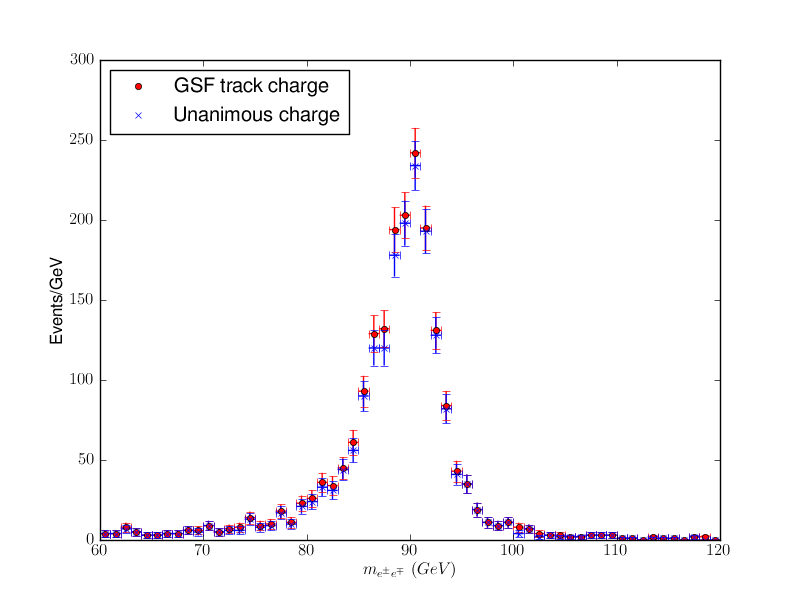
\includegraphics[width=0.85\textwidth]{zpeak_os}
    \caption{Oposite sign \PZ.}
    \label{fig:zpeak_os}
  \end{subfigure}
  \begin{subfigure}{\textwidth}
    \centering
    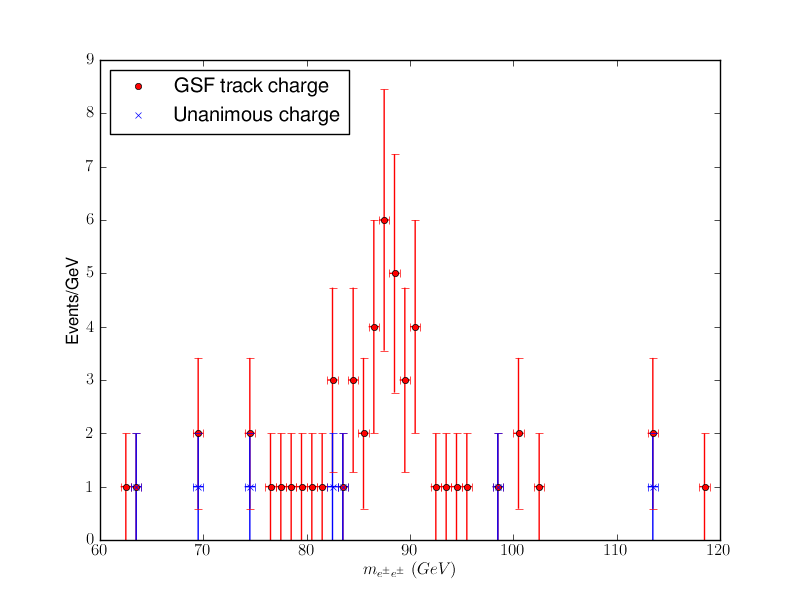
\includegraphics[width=0.85\textwidth]{zpeak_ss}
    \caption{Same sign \PZ.}
    \label{fig:zpeak_ss}
  \end{subfigure}
  \caption{ $Z\rightarrow ee$ peak. One electron is required to be in the
barrel to pass the VBTF80 selection and to have a fraction of energy loss by
radiation less than 0.3; the second electron is required only to pass the VBTF80
selection.}\label{fig:zpeak} 
\end{figure}

\subsection{Event Selection}
An Event is selected if it contains a single electron that passes all the electron
selection requirements.
To remove Drell-Yan events, an event is vetoed if it contains a second lepton
(an electron passing a loose selecton, or an isolated muon) with $\PT > 
\unit{15}{\GeV}$.

\section{Signal Yield Extraction Method}
The number of signal and background events in each bin is extracted using a fit
to the \ETm distribution using two templates.
The first is the sum of the \Wenu signal and the \ac{EWK} background shapes,
and the second is the sum of the \ac{QCD} plus \gjet processes.

\subsection{\ac{QCD} \ETm Shape}
The \ac{QCD} and \gjet background distribution is obtained from a control sample of
events. The control sample is selected by requiring that the electrons pass the
isolation and H over E cuts but fail the $\Delta\phi$ and $\Delta\eta$ cuts as
shown in \TableRef{asym36:antisel}.

\begin{figure}[htbp]
  \centering
  \begin{subfigure}{0.45\textwidth}
    \centering
    \includegraphics*[trim = 0mm 0mm 15mm 0mm, clip, width=\textwidth, angle=90]{MetCompare_anti_eta1.pdf}
    \caption{test.}
    \label{fig:qcd_met_eta1}
  \end{subfigure}
  \begin{subfigure}{0.45\textwidth}
    \centering
    \includegraphics*[trim = 0mm 0mm 15mm 0mm, clip, width=\textwidth, angle=90]{MetCompare_anti_eta2.pdf}
    \caption{test.}
    \label{fig:qcd_met_eta2}
  \end{subfigure}
  \begin{subfigure}{0.45\textwidth}
    \centering
    \includegraphics*[trim = 0mm 0mm 15mm 0mm, clip, width=\textwidth, angle=90]{MetCompare_anti_eta3.pdf}
    \caption{test.}
    \label{fig:qcd_met_eta3}
  \end{subfigure}
  \begin{subfigure}{0.45\textwidth}
    \centering
    \includegraphics*[trim = 0mm 0mm 15mm 0mm, clip, width=\textwidth, angle=90]{MetCompare_anti_eta4.pdf}
    \caption{test.}
    \label{fig:qcd_met_eta4}
  \end{subfigure}
  \begin{subfigure}{0.45\textwidth}
    \centering
    \includegraphics*[trim = 0mm 0mm 15mm 0mm, clip, width=\textwidth, angle=90]{MetCompare_anti_eta5.pdf}
    \caption{test.}
    \label{fig:qcd_met_eta5}
  \end{subfigure}
  \begin{subfigure}{0.45\textwidth}
    \centering
    \includegraphics*[trim = 0mm 0mm 15mm 0mm, clip, width=\textwidth, angle=90]{MetCompare_anti_eta6.pdf}
    \caption{test.}
    \label{fig:qcd_met_eta6}
  \end{subfigure}
  \caption{The \ETm distribution on antiselected \ac{MC} simulated events and selected \ac{QCD} and \gjet events in each pseudorapidity bin.}
  \label{asym36:antiselclosure}
\end{figure}

\begin{table}[htbp]
  \begin{center}
    \leavevmode
    \begin{tabular}{lcc} 
    \toprule
      \multicolumn{1}{c}{Variable} & \multicolumn{1}{c}{cut value (barrel)}& \multicolumn{1}{c}{cut value (endcap)}\\\midrule
        H/E & 0.04 & 0.025 \\
        $\Delta\phi$ & $>0.06$  & $>0.04$ \\
        $\Delta\eta$ & $>0.007$ & $>0.009$\\
        $ISO_{trk} / E_T $ & 0.09 & 0.04 \\
        $ISO_{ecal}/ E_T$  & 0.07 & 0.05 \\
        $ISO_{hcal}/ E_T$  & 0.10 & 0.025\\ 
    \bottomrule
    \end{tabular}
    \caption{\label{tab:AScuts}Electron anti-selection variables and corresponding cut values. $\Delta\phi$ and $\Delta\eta$ cuts are inverted.}
  \end{center}
\end{table}

To validate the antiselection used, \ac{QCD} \ac{MC} samples are used. The
distribution of \ac{QCD} events passing the event selection are comapred to the
antselected MC events. This is shown for each eta bin in
\FigureRef{asym36:antiselclosure}.

\subsection{Signal \ETm Shape from Boson Recoil}
The signal \ETm shape is obtained by modeling the recoil of the W boson. 
The recoil response and resolution in \HepProcess{\PZ\to\Plepton\Plepton} data
events is measured as a function of the \pT of the boson. This is combined with
information from the \PW and \PZ \ac{MC} simulation to derive a correction to
the simulation \ETm as a function of \PW \pT.

The modeling of the \HepProcess{\PW\to\Plepton\Pnu} \ETm with boson recoil is
described in detail here \cite{NULL}, and the ntuples containing
\HepProcess{\PW\to\Pelectron\Pnu} simulation with the recoil corrected \ETm were
provided from here \cite{NULL}.

\todo{ALOT MORE}

\subsection{\ac{EWK} \ETm Shape}
The EWK background processes that can produce a single isolated
electron which are considered in this analysis are:
\begin{itemize}
\item \HepProcess{\PZ\to\Pelectron\APelectron},
\item \HepProcess{\PZ\to\Ptauon\APtauon},
\item \HepProcess{\PW\to\Ptau\Pnu},
\item \HepProcess{\Ptop\APtop}.
\end{itemize}

The \ac{EWK} background \ETm distributions were obtained from Pythia \ac{MC}
simulations for each pseudorapidity/charge bin.  The scale of the \ac{EWK} shape
is fixed to the signal \ETm shape by the ratio obtained from \ac{MC} samples.

\subsection{Validation of Signal Extraction Method on Simulation}

The signal yield extraction procedure was validated using pseudodata
experiments. 1000 pseudodata experiments were generated with the number of
events expected in \unit{36.1}{\invpb} of data. The signal yields are extracted
in each experiment and the asymmetry is calculated. The distribution of
asymmetries is then fitted with a gaussian.

The width of the gaussian is the statistical uncertainty on the measurement.
The statistical uncertainty can also be estimated from the following formula
\begin{equation}
  \label{asym36:statuncert}
   \frac{d\mathcal{A}_{stat}}{d\eta} =
   \frac{2 \times \sqrt{ 
       \left( \frac{dN^+}{d\eta} \sigma_{\frac{dN^-} {d\eta}}\right)^2 + 
       \left( \frac{dN^-}{d\eta} \sigma_{\frac{dN^+} {d\eta}}\right)^2  }}
   {\left(  \frac{dN^+}{d\eta} +  \frac{dN^-}{d\eta} \right)^{2} } .
\end{equation}

The uncertainty from \EquationRef{asym36:statuncert} evaulated with \ac{MC} truth
values, and the uncertainty measured from pseudodata experiments for an
integrated luminosity of \unit{36.1}{\invpb} are summarised in
\TableRef{asym36:statuncertsum}.

\begin{table}[htbp]
  \begin{center}
    \begin{tabular}{lcc}
    \toprule
    $|\eta|$ range & $\sigma_{A}$ from \EquationRef{asym36:statuncert}. & $\sigma_{A}$ from pseudo-data exp.\\ \midrule
    $0.0<|\eta|<0.4$ & 0.0064 & 0.0062\\
    $0.4<|\eta|<0.8$ & 0.0064 & 0.0064\\
    $0.8<|\eta|<1.2$ & 0.0065 & 0.0065\\
    $1.2<|\eta|<1.4$ & 0.0096 & 0.0104\\
    $1.6<|\eta|<2.0$ & 0.0076 & 0.0079\\
    $2.0<|\eta|<2.4$ & 0.0077 & 0.0077\\
    \bottomrule
    \end{tabular}
  \caption{Expected statistical error as a function of pseudorapidity, for an
  integrated luminosity of \unit{36}{\invpb}. }
  \label{asym36:statuncertsum}
  \end{center}
\end{table}

%For each of the pseudo-data experiments we calulated the pull on the asymmetry measurement.
%The pull is defined as the diffence between the measured asymmetry for a pseudo-data experiment
%and the MC true value divided by the statistical uncertainty, and represents the number of standard deviations away from the true value.
%The distribution of the pulls from 1000 pseudo-data experiments are shown in figure \ref{fig:toyasym_pull}, and are fitted with a gaussian.
%It is expected that the mean of this gaussian is zero for an unbiased measurement and the
%sigma is one for a measurement with well understood statistical uncertainties.

\begin{figure}[htbp]
  \begin{center}
    \includegraphics*[angle=90,width=0.95\textwidth]{toyasym.pdf}
    \caption{\label{fig:toyasym}Measured Asymmetry for 1000 pseudo-data experiments. The distribution of the measured Asymmetry is fitted with a gaussian.}
  \end{center}
\end{figure}

\begin{figure}[htbp]
  \begin{center}
\includegraphics*[angle=90,width=0.95\textwidth]{pullasyTot.pdf}
    \caption{\label{fig:toyasym_pull}Pull on the Asymmetry in 1000 pseudo-data experiments. The distribution of the pull is fitted with a gaussian.}
  \end{center}
\end{figure}

\section{Corrections to the Measured Asymmetry}

To compare with the theoretical value, the measured lepton asymmetry has to be
corrected for experimental effects.

If the reconstruction efficiency of electrons is different to that of positrons
then a bias will be introduced in to the measured asymmetry.
The relative detection efficiency is the ratio of electron efficiency to the
positron efficiency,
\begin{equation}
 R = \epsilon^+/\epsilon^-
\end{equation}

If the relative effiecency, $R$, is not compatible with 1 it is necesary to
introduce a correction to the measured asymmetry.

\begin{equation}
\mathcal{A}_{exp}(\eta) = \frac{
                     \frac{dN}{d\eta}(e^+)- R\frac{dN}{d\eta}(e^-)
                     }
                     {
                     \frac{dN}{d\eta}(e^+)+ R\frac{dN}{d\eta}(e^-)
                     }
\end{equation}

The second experimental effect is due the charge missassignment of electrons.
The charge misassignment rate, $\omega$, is the rate at which electrons are
misasigned as positive charge and identified as positrons, and vice versa. The
misassignment induces a dilution factor to the asymmetry as a function of the
electron pseudorapidity. If it is assumed that the misassignment rate of
electrons to positrons is the same as the rate of positrons to electrons, \ie 

\begin{equation}
  \omega( \HepProcess{\APelectron \to \Pelectron} ) =
  \omega( \HepProcess{\Pelectron \to \APelectron} )
\end{equation}
then the dilution factor is given by $(1-2\omega_\eta)$ and the measured
asymmetry must be further corrected by the following relation
\begin{equation}
  \mathcal{A}_{exp}(\eta) = (1-2\omega_\eta)
                \frac{
                    \frac{dN}{d\eta}(e^+)-
                    R\frac{dN}{d\eta}(e^-)
                }
                {
                    \frac{dN}{d\eta}(e^+)+
                    R\frac{dN}{d\eta}(e^-)
                }
\end{equation}
which can be simplified to
\begin{align*}
  \mathcal{A}_{exp}(\eta) 
  &=
  \frac{1}{1-2\omega}
  \frac{ \mathcal{A}_M\left(R+1\right) - \left(R-1\right)}
       {\left(R+1\right)-\mathcal{A}_M \left(R-1\right)}\\
  &\simeq 
  \frac{1}{1-2\omega}
  \left(\mathcal{A}_M
 -\frac{\left(R-1\right)\left(1-\mathcal{A}_M^2\right)}{2}\right).
\end{align*}
where $\mathcal{A}_M$ is the uncorected measured asymmetry. The details of the
measurements of $R$ and $\omega$  are detailed with the results in the following
chapters.

\section{Other Systematic Effects}
There are several over systematic effects that must be evaluated and taken in to
account for the measurements.

The signal extraction procedure can may introduce some biases in to the measured
asymmetry. A bias may be introduced in to the measurement if there is a
difference between the \ETm templates used and the true \ETm distribution.  The
systematic uncertainties due to the signal extraction method are evaluated by
varying the templates used within certain uncertainties. The details are
described in more detail in the following chapters.

The energy resolution and scale of the electrons can introduce a systematic
error on the asymmetry due to the effect of of the transverse momentum cut
applied to the electrons. The largest source of electron scale bias is the
radiation induced change to the ECAL crystal transparency.
To correct fot this effect, energy scale and resolution corrrections are
derrived using a \Zee mass distribution. Te results are presented in the
following chapters.

